\subsection{Protection domain}
A protection domain(PD) is a concept of seL4. It is similar to a "process" on typical UNIX systems. 
However, by default a protection domain cannot do much and is completly isolated from all other protection domains.
Each PD consists of three components. It consists in minimum of one thread, a virtual address space(VSpace) and a capability space(CSpace).

\subsubsection{Threads}
For simplicity, each protection domain consists of exactly on thread.

\subsubsection{Virtual address space(VSpace)}
The complete virtual address space of each PD consists of two parts.
The lower part is the user space. The upper part is the kernel space.
The user space begins at address $us_b = 0$ and ends at address $us_e$. $us_e$ is defined
by $seL4$. For example: For RISC-V 64 it is define as $0x0000003ffffff000$.

\begin{tikzpicture}
    \tikzstyle{help lines}+=[dashed]
    \draw[style=help lines] (0,0) grid +(1,15);
    \node (us_b) at (-0.5, 0.2) {$us_b = 0$};
    \node (us) at (-0.5, 1.2) {4096};
    \node () at (-0.5, 2.3) {8192};
    \node (us_e) at (-0.5, 7.2) {$us_e = ks_b$};

    \draw[snake=brace] (us_b) -- (us_e);
    \node () [rotate=90] at (-1.0, 3.6) {User space};

    \node (ks_b) at (-0.5, 7.2) {};
    \node (ks_e) at (-0.5, 15.0) {};
    \draw[snake=brace] (ks_b) -- (ks_e);
    \node () [rotate=90] at (-1.0, 10.8) {Kernel space};
\end{tikzpicture}

\paragraph{Kernel space}


\paragraph{User space}

\begin{tikzpicture}
    \tikzstyle{help lines}+=[dashed]

    \draw[style=help lines] (0,0) grid +(1,20);
    \node (u_b) at (-0.5, 0.0) {0};
    \node (u_e) at (-0.5, 5.0) {};
    \draw[snake=brace] (u_b) -- (u_e);
    \node () [rotate=90] at (-1.0, 2.4) {thread independant};

    \node (heap_b) at (2.0, 5.0) {};
    \node (heap_e) at (2.0, 8.0) {};
    \node (heap_m) at (3.5, 6.5) {heap};
    \draw[snake=brace] (heap_e) -- (heap_b);

    \node (thread_0_b) at (2.0, 16.0) {};
    \node (thread_0_e) at (2.0, 20.0) {$t_{0_e}$};
    \node (thread_0_m) at (3.5, 18.0) {space thread 0};
    \draw[snake=brace] (thread_0_e) -- (thread_0_b);

    \node (thread_1_b) at (2.0, 12.0) {};
    \node (thread_1_e) at (2.0, 16.0) {$t_{1_e} = t_{0_b}$};
    \node (thread_1_m) at (3.5, 14.0) {space thread 1};
    \draw[snake=brace] (thread_1_e) -- (thread_1_b);

    \node (thread_n_b) at (2.0, 8.0) {$t_{n_b}$};
    \node (thread_n_e) at (2.0, 12.0) {$t_{n_e}$ };
    \node (thread_n_m) at (3.5, 10.0) {space thread n};
    \draw[snake=brace] (thread_n_e) -- (thread_n_b);
\end{tikzpicture}
The space size $s_{max}$ is for every thread the same.
$s_{max} = 512$ pages. the page size $s_p  = 4096$ bytes.
\begin{equation}
    b = s_{max} * s_p \\\\
\end{equation}
\begin{equation}
    r = u_{e_{seL4}} - b \left \lfloor \frac{u_{e_{seL4}}}{b} \right \rfloor
\end{equation}
\begin{equation}
    u_e = u_{e_{seL4}} - r
\end{equation}
It can be simplified to
\begin{equation}
    u_e = b \left \lfloor \frac{u_{e_{seL4}}}{b} \right \rfloor
\end{equation}
The end of the space of thread $n$ is defines as
\begin{equation}
    s_{e_n} = u_e - n * b
\end{equation}
The lowest page is not mapped and is used as guard page to protect against stack clash.
The beginnng of the stack of thread $n$ is defined as
\begin{equation}
    s_{b_n} = u_e - (n + 1) * b
\end{equation}
The address space from $s_{b_n}$ to $s_{b_n} + s_p - 1$ is not usable, as it is used
as stack protection.


\begin{figure}
    \label{fig:thread_space}
    \begin{tikzpicture}
        \tikzstyle{help lines}+=[dashed]

        \draw[style=help lines] (0,0) grid +(10,1);
        \node (u_b) at (0.2, 1.2) {$t_{n_b}$};
        \node (u_e) at (1.2, 1.2) {$t_{n_b}$};
        \node () at (0.5, 0.5) {TCB};
        \node () at (1.5, 0.5) {IPC};

        \node (thread_n_b) at (2.2, 1.2) {$t_{n_b}$};
        \node (thread_n_e) at (10.2, 1.2) {$t_{n_e}$ };
        \node () at (6.0, 1.5) {Stack};
        \draw[snake=brace] (thread_n_b) -- (thread_n_e);
    \end{tikzpicture}
\end{figure}

TCB: Is only virtually mapped.
Means, that the capability is stored in the cap space, where the cap to the correspondig
page would be stored.

IPC: 


\paragraph{RISCV SV39}
Virtual address

3 Level
Every level $2^9$ entries and translate 9 bits.
Page size: $2^12$ bytes

\begin{tikzpicture}
    \tikzstyle{help lines}+=[dashed]

    \draw[style=help lines] (0,0) grid +(5,1);
    \node(n_0_b) at (0.5, 0.5) {};
    \node() at (-0.5, 0.5) {v};
    \node () at (0.5, 0.5) {$v_{0}$};
    \node() at (2.5, 0.5) {$v_i$};
    \node () at (4.5, 0.5) {$v_{511}$};

    \node(n_0_e) at (-2.5, -2.5) {};
    \draw [->] (n_0_b) -- (n_0_e);

    \draw[style=help lines] (-3, -3) grid +(5,1);
    \node(n_00_b) at (-2.5, -2.5) {};
    \node(n_00_e) at (-4.5, -5.5) {};
    \node() at (-3.5, -2.5) {$v_{0}$};
    \node () at (-2.5, -2.5) {$v_{00}$};
    \node () at (-0.6, -2.5) {$v_{ij}$}; 
    \node () at (1.5, -2.5) {$v_{0511}$};
    \draw [->] (n_00_b) -- (n_00_e);

    \draw[style=help lines] (3, -3) grid +(5,1);

    \draw[style=help lines] (-5, -6) grid +(5,1);
    \node () at (-4.5, -5.5) {$v_{000}$};
    \node () at (-2.5, -5.5) {$v_{ijk}$};
    \node () at (-0.5, -5.5) {$v_{00511}$};

    \draw[style=help lines] (5, -6) grid +(5,1);

    \draw[style=help lines] (-5, -9) grid +(14, 1);
    \node(p_0) at (-4.8, -7.8) {0};
    \node(p_1) at (-3.8, -7.8) {4096};
    \node(p_3) at (-2.8, -7.8) {8192};

\end{tikzpicture}


\subsubsection{Capability space(CSpace)}
Each protection domain has its own capability space, which is a data structure that holds all capabilities that a PD has access to.
A PDs is not able to access anything unless it is explicitly allow to do it. This is allowed by the capability system, as all resources in seL4 are modelled by capabilities. 
If a PD does not have the capability to some resource, seL4 does not allow it to use it.

\begin{figure}
    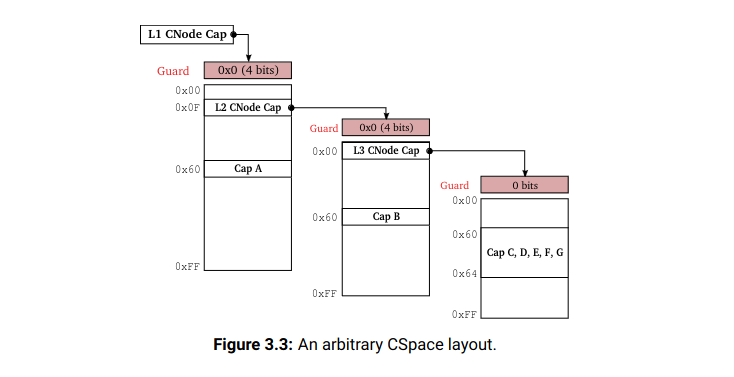
\includegraphics[scale=0.5]{./figures/seL4_cap_space_addresssing.png}
    \label{asdfasd}
\end{figure}

"A capability address is stored in a CPointer (abbreviated CPtr), which is an unsigned integer
variable. Capabilities are addressed in accordance with the translation algorithm described
above. Two special cases involve addressing CNode capabilities themselves and addressing a
range of capability slots.
Recall that the translation algorithm described above will traverse CNode capabilities while there
are address bits remaining to be translated. Therefore, in order to address a capability which
may be a CNode capability, the user must supply not only a capability address but also specify
the maximum number of bits of the capability address that are to be translated, called the depth
limit. When a CPointer is paired with depth limit depth, only its depth least significant bits are
used in translation.
Certain methods, such as $seL4_Untyped_Retype()$, require the user to provide a range of capa-
bility slots. This is done by providing a base capability address, which refers to the first slot in the
range, together with a window size parameter, specifying the number of slots (with consecutive
addresses, following the base slot) in the range.
Figure 3.3 depicts an example CSpace. In order to illustrate these ideas, we determine the ad-
dress of each of the 10 capabilities in this CSpace.
Cap A. The first CNode has a 4-bit guard set to 0x0, and an 8-bit radix. Cap A resides in slot
0x60 so, provided that it is not a CNode capability, it may be referred to by any address
of the form 0x060nnnnn (where nnnnn is any sequence of 5 hexadecimal digits, because
the translation process terminates after translating the first 12 bits of the address). For
simplicity, we usually set unused address bits to 0, which in this case yields the address
0x06000000.
Cap B. Again, the first CNode has a 4-bit guard set to 0x0, and an 8-bit radix. The second CNode
is reached via the L2 CNode Cap. It also has a 4-bit guard of 0x0 and Cap B resides at index
0x60. Hence, Cap B’s address is 0x00F06000. Translation of this address terminates after
the first 24 bits.
Cap C. This capability is addressed via both CNodes. The third CNode is reached via the L3
CNode Cap, which resides at index 0x00 of the second CNode. The third CNode has no
guard and Cap C is at index 0x60. Hence, its address is 0x00F00060. Translation of this
address leaves 0 bits untranslated.
Caps C–G. This range of capability slots is addressed by providing a base address (which refers
to the slot containing Cap C) of 0x00F00060 and a window size of 5.
L2 CNode Cap. Recall that to address a CNode capability, the user must supply not only a ca-
pability address but also specify the depth limit, which is the maximum number of bits to
16 CHAPTER 3. CAPABILITY SPACES
be translated. L2 CNode Cap resides at offset 0x0F of the first CNode, which has a 4-bit
guard of 0x0. Hence, it may be referred to by any address of the form 0xnnnnn00F with a
depth limit of 12 bits, where nnnnn is any sequence of 5 hexadecimal digits.
L3 CNode Cap. This capability resides at index 0x00 of the second CNode, which is reached by
the L2 CNode Cap. The second CNode has a 4-bit guard of 0x0. Hence, the capability may
be referred to by any address of the form 0xnn00F000 with a depth limit of 24 bits, where
nn is any sequence of 2 hexadecimal digits.
In summary, to refer to any capability (or slot) in a CSpace, the user must supply its address.
When the capability might be a CNode, the user must also supply a depth limit. To specify a
range of capability slots, the user supplies a starting address and a window size.\cite{seL4:2024}" 


$4096 / 32 = 128$

\begin{tikzpicture}
    \tikzstyle{help lines}+=[dashed]

    \draw[style=help lines] (0,0) grid +(10,1);

    \node(n_0_b) at (0.5, 0.5) {};
    \node () at (0.2, 1.2) {0};
    \node() at (9.2, 1.2) {127};

    \node(c_0) at (2.5, 0.5) {$c_{0}$};
    \node() at (3.5, 0.5) {$c_{v}$};
    
\end{tikzpicture}


PD does not have the capability to manipulate its own CSpace, consequently neither its Vspace.
